\documentclass[11pt,a4paper]{article}
\usepackage[T1]{fontenc}
\usepackage[utf8]{inputenc}
\usepackage{lmodern}
\usepackage[a4paper,margin=25mm,headheight=15pt]{geometry}
\usepackage{amsmath,amssymb,amsthm,mathtools}
\usepackage{microtype}
\usepackage{booktabs,tabularx,array,longtable}
\usepackage{graphicx,xcolor}
\usepackage{enumitem}
\usepackage{fancyhdr}
\usepackage{xurl}
\definecolor{accent}{HTML}{165C67}
\definecolor{ink}{HTML}{19303D}
\usepackage[colorlinks=true,linkcolor=accent,citecolor=accent,urlcolor=accent,
  pdftitle={Exact Cubic Euler-Factor Matching and Optimal Unequal-Precision Recovery},
  pdfauthor={Prepared with ChatGPT},bookmarksnumbered=true]{hyperref}
\usepackage{bookmark}
\urlstyle{same}
\setcounter{tocdepth}{1}
\setlist[enumerate]{leftmargin=*,itemsep=0.4em,topsep=0.4em}
\setlist[itemize]{leftmargin=*,itemsep=0.25em,topsep=0.4em}
\newtheorem{theorem}{Theorem}[section]
\newtheorem{lemma}[theorem]{Lemma}
\newtheorem{proposition}[theorem]{Proposition}
\newtheorem{corollary}[theorem]{Corollary}
\theoremstyle{definition}
\newtheorem{definition}[theorem]{Definition}
\theoremstyle{remark}
\newtheorem{remark}[theorem]{Remark}
\newcommand{\F}{\mathbb F}
\newcommand{\C}{\mathbb C}
\newcommand{\Z}{\mathbb Z}
\newcommand{\Q}{\mathbb Q}
\newcommand{\E}{\mathbb E}
\newcommand{\abs}[1]{\lvert#1\rvert}
\newcommand{\norm}[1]{\lVert#1\rVert}
\DeclareMathOperator{\supp}{supp}
\DeclareMathOperator{\ord}{ord}
\newcommand{\code}[1]{\texttt{\small #1}}
\newcolumntype{L}[1]{>{\raggedright\arraybackslash}p{#1}}
\newcolumntype{Y}{>{\raggedright\arraybackslash}X}
\pagestyle{fancy}
\fancyhf{}
\fancyhead[L]{\small\sffamily Cubic matching and unequal precision}
\fancyhead[R]{\small\sffamily Research report}
\fancyfoot[C]{\thepage}
\renewcommand{\headrulewidth}{0.3pt}
\setlength{\parskip}{0.25em}
\emergencystretch=2em
\allowdisplaybreaks[1]

\title{Exact Cubic Euler-Factor Matching\\[4pt]
and Optimal Unequal-Precision Recovery}
\author{A source-pinned research report prepared with ChatGPT}
\date{27 November 2026}
\begin{document}
\hypersetup{pageanchor=false}
\begin{titlepage}
\thispagestyle{empty}
{\color{accent}\sffamily\bfseries RESEARCH REPORT\par}
\vspace{1.5cm}
{\sffamily\bfseries\fontsize{27}{33}\selectfont
Exact Cubic\\Euler-Factor Matching\par}
\vspace{0.5cm}
{\sffamily\fontsize{22}{28}\selectfont
and Optimal Unequal-Precision Recovery\par}
\vspace{0.8cm}
{\large Two extensions of the supplied Dirichlet-GRH development\\
and its companion article\par}
\vspace{1cm}
\hrule
\vspace{0.65cm}
\begin{abstract}
We prove an exact extremal theorem for products of cubic Dirichlet
$L$-functions: for every packet size and character-group rank, we determine
the smallest density of primes with different Euler factors and classify
all pairs attaining it. An integral Fourier transform, reduction at the
Eisenstein prime above three, and the first two ternary Reed--Muller
weights produce a two-step extremal function. The density and rigidity
theorems are unconditional. The supplied Dirichlet GRH gives finite-prime
detection and a uniform smoothed count for all extremizers.

Separately, we determine the exact kernel of formal-series observations
along branches recorded to unequal precisions. This yields sharp jet
recovery, error/erasure thresholds, a contact-tree algorithm, and optimal
recording budgets. It resolves the field-valued unequal-length portion
of an explicit question in the supplied article.

The report includes complete proofs, an audit of the pinned source and
its theorem scope, exact computational checks, and reproducibility files.
These new results have not been formalized in Lean. Novelty is assessed
against the supplied collection and targeted primary-literature searches;
worldwide priority is not asserted.
\end{abstract}
\vfill
{\sffamily 27 November 2026\par}
\medskip
{\small Source snapshot:\\
\texttt{ProveIt}\quad\texttt{2a9f8e3ee74a1824d57546f0b1b4f1cef5df93d6}\par}
\end{titlepage}
\hypersetup{pageanchor=true}
\pagenumbering{roman}
\tableofcontents
\bigskip
\noindent\textbf{Reading guide.}
Section~\ref{sec:source} fixes the source and its scope.
The main mathematical results are Theorems~\ref{thm:cubic-min}
and~\ref{thm:cubic-equality}; Section~\ref{sec:example} makes them
explicit at modulus $1729$.
Section~\ref{sec:unequal-branches} is an independent second extension.
Section~\ref{sec:verification} separates proofs, finite checks, and
unperformed formal verification.
\clearpage
\pagenumbering{arabic}
\section{Scope, source assessment, and contributions}\label{sec:source}

\subsection{Exactly which source was analyzed}

The supplied paths were read at ProveIt commit
\begin{center}
\texttt{2a9f8e3ee74a1824d57546f0b1b4f1cef5df93d6}.
\end{center}
This pins the analysis even if the repository later changes. The two inputs
are the vendored readable Lean development \cite{vendor,sernau} and
\emph{Beyond the Riemann hypothesis for Dirichlet $L$-functions:
consequences, transfers and limits} \cite{article}.

The complete Git tree of the vendored \code{grh/} directory is
\begin{center}
\texttt{2e133df63d7f4da6b3059c4195324f8e9187ba73}.
\end{center}
It equals the upstream \code{grh/} tree at
\code{72fead102f663d5c7a407964a13dc0cf9d977207}, as checked against the
upstream GitHub tree response. There are 818 files in that directory and
803 Lean modules below \code{src/}. The local import closure of
\code{Main.lean} contains all 803 modules. The package pins Lean
\code{v4.35.0} and Mathlib
\code{56a005855ea17e0b0958f73ec801ae140b0a1679}.

A lexical audit, after removing nested comments and strings, found no
\code{sorry}, \code{admit}, \code{axiom}, \code{unsafe},
\code{native\_decide}, or \code{implemented\_by} code tokens in this
closure. The deliberately incomplete \code{Challenge.lean} is a separate,
unimported statement-comparison target; its placeholders are not part of
the proof closure. This audit does not by itself validate the proof.

No Lean build or independent kernel replay was run in this session.
Andrew Sutherland's verification page for the same upstream commit reports
successful builds, statement and axiom checks, complete kernel replay,
and independent checker acceptance for the readable and compact editions
\cite{sutherland}. Those are external verification reports. Also, a build
of the ProveIt repository root does not build this separately pinned
vendored package; its own directory and toolchain must be used
\cite{vendor}.

\subsection{The exact mathematical input}

The source statement file imports only Mathlib. Its five exported results
include Mathlib's ordinary Riemann hypothesis and Dirichlet GRH with the
following scope:
\begin{enumerate}
\item Every zero of the Riemann zeta function other than the negative even
integers lies on $\Re s=1/2$, with the conventionally valued pole point
$s=1$ explicitly excluded in the total-function formulation.
\item For every positive modulus and every complex Dirichlet character,
$L(s,\chi)\ne0$ when $\Re s>1/2$, apart from the principal character's
pole at $s=1$.
\item Every Dirichlet $L$-function zero in the open critical strip lies on
$\Re s=1/2$. This includes imprimitive characters; there is also a
primitive-character specialization.
\end{enumerate}
These are the declarations in \code{Statements.lean} and \code{Main.lean}
at the pinned revision \cite{sernau}. The conclusion concerns Dirichlet
$L$-functions over $\Q$. It does not quantify over arbitrary automorphic
$L$-functions, nonabelian Artin $L$-functions, or all number-field zeta
functions, and it imposes no simplicity condition on critical-line zeros.
Every use of GRH in this report fits the stated Dirichlet scope.

\subsection{How the proof mechanism leads to these extensions}

The readable reduction compares upper and lower estimates for the same
corrected covolume. Short integral theta-derived forms give an upper
estimate; near-full-rank spanning supplies enough vectors; a product formula
for twisted lattices, with controlled denominators and torsion
specializations, gives a lower estimate. The common height cancels. In the
source notation the resulting estimate is
\[
 m\cdot\mathrm{totalRemainder}\le f a(\log b)^5.
\]
The reduction files then turn this into an eventual one-sided estimate for
a smoothed prime remainder. An analytic pole-exclusion argument gives
nonvanishing to the right of the critical line, and the functional equation
gives the critical-strip conclusion. These roles can be traced directly in
\code{New/Reduction/MainInequality.lean},
\code{New/Reduction/OneSidedBound.lean}, and \code{New/Main.lean}
\cite{sernau}.

The companion article develops two useful interfaces from this setting.
One identifies products of Dirichlet $L$-functions from their prime data;
the other studies information retained by specialization along highly
contacting formal branches. We extend those interfaces rather than
asserting that an arbitrary nonabelian GRH follows from the input.

The first extension starts from the article's quadratic matching theorem
\code{rec:thm:qmatch}. Its open-question paragraph asks for analogous
matching densities for odd-prime-order characters. The quadratic reduction
uses an integral Walsh transform. At order three, the correct local ring is
the Eisenstein ring at $1-\zeta_3$. Complex conjugation adds a symmetry that
forces the second ternary coding weight in one of the two size regimes.
Section~\ref{sec:cubic} proves the exact extremal cubic result and every
equality case. It does not determine the entire nonextremal density
spectrum or the case of every odd prime exponent.

The second extension starts from the equal-length branch kernel, distance,
and pruning results \code{lub:thm:kernel}, \code{lub:thm:distance}, and
\code{lub:thm:dp}. Question \code{lub:q:adversarial} explicitly asks for
unequal observation lengths, higher uniformizer-power coefficient rings,
and faster error-location methods. Section~\ref{sec:unequal-branches}
resolves the unequal-length field case and its optimal recording costs.
The coefficient-ring and fast-decoding parts remain outside the result.

\subsection{Dependency and novelty map}

\begin{center}
\small
\begin{tabularx}{\linewidth}{@{}L{0.32\linewidth}YL{0.23\linewidth}@{}}
\toprule
Result proved here & Contribution & Analytic dependence\\
\midrule
Exact cubic minimum and all extremizers & Sharp extremal answer for every
$r,k$; new extension of \code{rec:thm:qmatch} & Unconditional; standard
Reed--Muller inputs\\[4pt]
Cubic erasure/corruption thresholds & Sharp consequences of that minimum &
Unconditional\\[4pt]
Finite distinguishing primes and extremal counting & General Fourier bound;
exact extremal indicator norms $4/3,16/9$ & Uses supplied Dirichlet GRH\\[4pt]
Unequal-length kernel and jet recovery & Exact formal-series ambiguity and
recovery criterion & Unconditional\\[4pt]
Branch deletion, distance, and budgets & Exact pruning recursion and sharp
clean/maximal-distance costs & Unconditional\\
\bottomrule
\end{tabularx}
\end{center}

The source article describes itself as a merge of 120 reports, containing
869 results across 689 pages, without a fresh independent review of every
claim \cite{article}. This session inspected the source theorem and the
relevant matching and branch-recovery arguments; it did not certify all
869 results. The present proofs are given in full modulo explicitly cited
standard coding and analytic inputs. The coding weight theorems,
$P$-orderings, weighted greedy selection, and the usual distance criterion
are established tools, not claimed discoveries.

\section{The exact cubic matching theorem}\label{sec:cubic}

The article asks whether its quadratic Euler-factor matching results have an
analogue for characters of odd prime order \cite{article}. We determine the
minimum disagreement density for characters of order dividing three, for every
packet size and every rank, and classify every pair attaining that minimum.
The resulting function has two different steps between successive powers of
three. The extremal configurations also give exact erasure and corruption
thresholds for identifying a product from its local factors.

\subsection{Packets and the extremal function}

Let $X$ be a group of Dirichlet characters modulo $Q$, of exponent three and
rank $r\geq1$. Thus $X\simeq\F_3^r$. The principal character belongs to $X$.
We write the group law on $X$ additively when describing its subspaces and
cosets. A \emph{packet} $A$ is a multiset of $k\geq1$ members of $X$, and its
local polynomial at $p\nmid Q$ is
\[
 P_A(p,T)=\prod_{\chi\in A}(1-\chi(p)T).
\]
For distinct packets $A,C$ of the same size, let $\delta(A,C)$ be the natural
density, among rational primes, of the set on which $P_A(p,T)\ne P_C(p,T)$.
Write $\Delta_{r,k}$ for the minimum of these densities over all such pairs.

\begin{theorem}[Exact minimum disagreement]\label{thm:cubic-min}
The density $\delta(A,C)$ exists. Put $a=\lfloor\log_3 k\rfloor$. Then
\begin{equation}\label{eq:cubic-min}
 \Delta_{r,k}=
 \begin{cases}
  2/3^r,&k\geq3^{r-1},\\[2pt]
  2/3^{a+1},&a\leq r-2,\quad 3^a\leq k<2\cdot3^a,\\[2pt]
  4/3^{a+2},&a\leq r-2,\quad 2\cdot3^a\leq k<3^{a+1}.
 \end{cases}
\end{equation}
The theorem is unconditional.
\end{theorem}

For example, at rank at least three, the least disagreement densities for
$k=1,2,3,4,5,6,7,8,9$ are respectively
\[
 \frac23,\quad\frac49,\quad\frac29,\quad\frac29,\quad\frac29,
 \quad\frac4{27},\quad\frac4{27},\quad\frac4{27},\quad\frac2{27}.
\]
Consequently two distinct products of six factors can have identical local
polynomials at a proportion $23/27$ of the primes, and no larger proportion
is possible. With nine factors the optimal proportion is $25/27$.

For the classification, cancel common entries of $A$ and $C$, and write
\[
 c(\chi)=m_A(\chi)-m_C(\chi),\qquad
 b=\sum_{c(\chi)>0}c(\chi)=\frac12\sum_\chi\abs{c(\chi)}\leq k.
\]
Here $b$ is the size of either packet after cancellation.

\begin{theorem}[All extremizers]\label{thm:cubic-equality}
Every pair attaining \eqref{eq:cubic-min} has the following form, up to
interchanging the two packets and adding the same multiset to both.
\begin{enumerate}
\item If $a\leq r-2$ and $3^a\leq k<2\cdot3^a$, there are a subspace
  $U\leq X$ of dimension $a$, an element $\eta\in X$, and $\theta\notin U$
  such that the reduced packets are
  \[
   A=\eta+U,\qquad C=\eta+\theta+U.
  \]
  In particular, $b=3^a$ and neither reduced packet has repeated entries.
\item If $a\leq r-2$ and $2\cdot3^a\leq k<3^{a+1}$, there are a subspace
  $U\leq X$ of dimension $a$, an element $\eta\in X$, and $\alpha,\beta$
  linearly independent modulo $U$ such that
  \begin{align*}
   A&=(\eta+\alpha+U)\mathbin{\dot\cup}(\eta-\alpha+U),\\
   C&=(\eta+\beta+U)\mathbin{\dot\cup}(\eta-\beta+U).
  \end{align*}
  Here $b=2\cdot3^a$, again without repetitions.
\item If $k\geq3^{r-1}$, there is a hyperplane $U<X$ such that $c$ is
  constant on its three cosets. Its three integer values $d_0,d_1,d_2$
  satisfy
  \[
   d_0+d_1+d_2=0,\qquad(d_0,d_1,d_2)\ne(0,0,0),\qquad
   b=3^{r-1}\max_j\abs{d_j}\leq k.
  \]
  Every such coefficient function is an extremizer.
\end{enumerate}
Conversely every displayed construction attains the stated minimum.
\end{theorem}

The third case covers $r=1$ and every $k\geq1$. The theorem concerns the exact
extremal function and its complete equality classification. The other
attainable densities form a further classification problem.

\begin{corollary}[Characters of exact order three]\label{cor:cubic-nonprincipal}
Formula~\eqref{eq:cubic-min} remains valid if every packet entry must be
nonprincipal, hence of exact order three.
\end{corollary}

\begin{proof}
The lower bound already applies to this restricted family. For the lower
construction use the two cosets $\theta+U$ and $-\theta+U$, where
$\theta\notin U$; neither contains the identity. For the upper
construction the four cosets $\alpha+U$, $-\alpha+U$, $\beta+U$ and
$-\beta+U$ already avoid the identity. At saturation take the two
nonzero cosets of a hyperplane. Pad both packets by the same nonprincipal
character as necessary; one exists because $r\geq1$. This also handles
$r=1$. The equality classification is the restriction of
Theorem~\ref{thm:cubic-equality} to configurations and common fillers
that avoid the identity.
\end{proof}

\subsection{From local factors to an integral Fourier transform}

Fix $\zeta=e^{2\pi i/3}$, and let
$V=\operatorname{Hom}(X,\{1,\zeta,\zeta^2\})\simeq\F_3^r$.
For $v\in V$ write $\chi(v)$ for evaluation. Define
\begin{equation}\label{eq:cubic-H}
 H(v)=\sum_{\chi\in X}c(\chi)\chi(v).
\end{equation}
Finite Fourier inversion shows that $H\ne0$. Also
\begin{equation}\label{eq:cubic-symmetry}
 H(0)=0,\qquad H(-v)=\overline{H(v)}.
\end{equation}

\begin{lemma}[Trace detects the whole cubic local polynomial]
\label{lem:cubic-trace}
At every $v\in V$, equality of the two traces is equivalent to equality of
the two local polynomials. Moreover
\begin{equation}\label{eq:cubic-density}
 \delta(A,C)=3^{-r}\abs{\supp H}.
\end{equation}
\end{lemma}

\begin{proof}
Let
\[
 C_j(v)=\sum_{\chi(v)=\zeta^j}c(\chi)\qquad(j=0,1,2).
\]
Then $\sum_jC_j(v)=0$ and
$H(v)=C_0(v)+C_1(v)\zeta+C_2(v)\zeta^2$.
The minimal polynomial $1+Z+Z^2$ implies that this expression vanishes
precisely when $C_0(v)=C_1(v)=C_2(v)$; their zero sum then makes all three
zero. This says exactly that the multiplicities of the three possible
local roots agree.

The evaluation homomorphism $(\Z/Q\Z)^\times\to V$ is surjective. Indeed,
the annihilator of its image in $X$ consists of the character trivial on
every reduced residue class, which is the identity character. A proper
subgroup of a finite elementary abelian group has a nontrivial annihilator.
All fibers therefore have the same size. The prime number theorem in
arithmetic progressions gives \eqref{eq:cubic-density}.
\end{proof}

\subsection{The Eisenstein valuation and the degree bound}

Put $R=\Z[\zeta]$ and $\varpi=1-\zeta$. We use
\[
 \varpi^2=-3\zeta,\qquad R/(\varpi)\simeq\F_3,
 \qquad\overline\varpi=-\zeta^2\varpi.
\]
For a nonzero element of $R$, let $v_{\varpi}$ be its divisibility order at
$\varpi$. Set
\[
 t=\min_{H(v)\ne0}v_{\varpi}(H(v)),\qquad
 f(v)=\varpi^{-t}H(v)\pmod\varpi.
\]
The function $f:V\to\F_3$ is nonzero. Since all character values are
$1\pmod\varpi$ and $\sum c(\chi)=0$, one has $t\geq1$.

\begin{lemma}[Low degree after dividing by the common valuation]
\label{lem:cubic-degree}
The reduced polynomial representing $f$ on $\F_3^r$ has total degree at most
$t$. In addition,
\begin{equation}\label{eq:cubic-fparity}
 f(0)=0,\qquad f(-v)=(-1)^t f(v),\qquad\supp f\subseteq\supp H.
\end{equation}
\end{lemma}

\begin{proof}
Represent each coordinate by $0,1,2$. For $e\in\{0,1,2\}$ the polynomial
\[
 1+(\zeta^e-1)x+(\zeta^e-1)^2\frac{x(x-1)}2
\]
interpolates $x\mapsto\zeta^{ex}$ on these three representatives. Its
coefficient of $x^j$ is divisible by $\varpi^j$, for $j=0,1,2$, in
$R[1/2]$. Taking products in the coordinates and integer linear
combinations produces the reduced interpolating polynomial for $H$;
every coefficient of total degree $j$ is divisible by $\varpi^j$.

Every coefficient is also divisible by $\varpi^t$. To see this, interpolate
the values $\varpi^{-t}H(v)$ instead. The one-variable evaluation matrix
on $0,1,2$ has determinant $2$, so its inverse, and the tensor product
inverse in $r$ variables, have entries in $R[1/2]$. Thus division of the
interpolating polynomial by $\varpi^t$ leaves its coefficients in
$R[1/2]$. Reducing modulo $\varpi$ kills every monomial of degree greater
than $t$, proving the degree claim.

The support and value at zero follow from the definition. Conjugation
acts trivially on $R/(\varpi)$, while
$\overline\varpi/\varpi=-\zeta^2\equiv-1\pmod\varpi$.
Equation \eqref{eq:cubic-symmetry} therefore gives the parity identity.
\end{proof}

\begin{lemma}[Exact cost of an odd or even valuation]
\label{lem:cubic-cost}
If $t=2j+1$, then $b\geq3^j$. If $t=2j+2$, then $b\geq2\cdot3^j$.
\end{lemma}

\begin{proof}
Choose $v$ attaining the minimum defining $t$, and abbreviate $C_j(v)$ to
$C_j$. For any zero-sum integer triple the positive mass is its largest
absolute entry. Coalescing the coefficients of $c$ into this triple
cannot increase its positive mass, so
\[
 \max_j\abs{C_j}\leq b.
\]
Factor the largest common power $3^m$ from $(C_0,C_1,C_2)$, obtaining a
zero-sum integer triple $(n_0,n_1,n_2)$ not all divisible by three. Its
residue triple is either a permutation of $(0,1,2)$, or has three equal
nonzero entries.

In the first case,
$n_0+n_1\zeta+n_2\zeta^2$ is divisible by $\varpi$ but not by
$\varpi^2$, because its two coefficients in the basis $1,\zeta$ are not
both divisible by three. Thus $t=2m+1$ and
$b\geq3^m$.

In the second case put $A=n_0-n_2$, $B=n_1-n_2$. Both are divisible by
three, whereas
\[
 \frac{A+B}{3}=-n_2\not\equiv0\pmod3.
\]
Consequently $(A+B\zeta)/3$ is not divisible by $\varpi$, so $t=2m+2$.
Three integers with a common nonzero residue modulo three and zero sum
cannot all have absolute value at most one. Hence
$b\geq2\cdot3^m$.
\end{proof}

\subsection{The coding input and the minimum}

We use these established Reed--Muller facts
\cite{leducq2012,leducq2010}. On $\F_3^r$, nonzero reduced polynomials of
degree at most $2j+1<2r$ have support at least
$2\cdot3^{r-j-1}$. At degree at most $2j<2r$, the minimum is $3^{r-j}$,
and minimum supports are affine subspaces of codimension $j$. For
$1\leq j\leq r-1$, the next weight is $4\cdot3^{r-j-1}$; each support
of that weight is contained in an affine subspace of codimension $j-1$.
Minimum supports at odd degree lie in an affine subspace of codimension
$j$. The second-weight formula at degree two includes $r=2$.

\begin{lemma}[The symmetry excludes the even minimum]
\label{lem:cubic-weight}
For the function $H$ in \eqref{eq:cubic-H}, the following bounds hold:
\begin{align}
 t=2j+1<2r&\quad\Longrightarrow\quad
  3^{-r}\abs{\supp H}\geq\frac2{3^{j+1}},\label{eq:cubic-odd}\\
 t=2j<2r&\quad\Longrightarrow\quad
  3^{-r}\abs{\supp H}\geq\frac4{3^{j+1}}.
  \label{eq:cubic-even}
\end{align}
In all cases $3^{-r}\abs{\supp H}\geq2/3^r$.
\end{lemma}

\begin{proof}
For odd $t$, apply the minimum-weight bound to $f$ and use
$\supp f\subseteq\supp H$. For even $t=2j$, a minimum-weight $f$ would
have support an affine subspace $A$ of codimension $j$.
Equation \eqref{eq:cubic-fparity} gives $A=-A$. An affine subspace over
$\F_3$ invariant under negation contains zero: it contains the midpoint
of any $v$ and $-v$. This contradicts $f(0)=0$. The second-weight bound
therefore applies. Finally $\supp H$ is nonempty, invariant under
negation, and excludes zero, so it contains at least one pair
$\{v,-v\}$.
\end{proof}

\begin{proof}[Proof of Theorem~\ref{thm:cubic-min}]
The density formula is Lemma~\ref{lem:cubic-trace}. First suppose
$a\leq r-2$ and $3^a\leq k<2\cdot3^a$. Lemma~\ref{lem:cubic-cost}
forces $t\leq2a+1$. An odd value $t=2j+1$ has $j\leq a$, and
\eqref{eq:cubic-odd} gives $\delta(A,C)\geq2/3^{a+1}$.
An even value $t=2j$ has $j\leq a$ and gives the strictly larger bound
$4/3^{a+1}$.

If $a\leq r-2$ and $2\cdot3^a\leq k<3^{a+1}$, the cost lemma forces
$t\leq2a+2$. The weakest bound is now at $t=2a+2$, giving
$4/3^{a+2}$; every smaller $t$ gives a larger bound. If
$k\geq3^{r-1}$, use the universal two-point bound.

For sharpness choose a subspace $U\leq X$ of dimension $a$ and
$\theta\notin U$. The packets $U$ and $\theta+U$ have size $3^a$ and
Fourier difference
\begin{equation}\label{eq:cubic-construct-odd}
 H(v)=3^a\mathbf1_{U^\perp}(v)(1-\theta(v)).
\end{equation}
Its support has relative size $3^{-a}(2/3)$.
For the other range choose $\alpha,\beta$ independent modulo $U$ and
take the two packets
$(\alpha+U)\mathbin{\dot\cup}(-\alpha+U)$ and
$(\beta+U)\mathbin{\dot\cup}(-\beta+U)$.
For $v\in U^\perp$, write $\alpha(v)=\zeta^x$ and
$\beta(v)=\zeta^y$. Then
\begin{equation}\label{eq:cubic-construct-even}
 H(v)=3^{a+1}\bigl(\mathbf1_{x=0}-\mathbf1_{y=0}\bigr).
\end{equation}
Exactly one of $x,y$ vanishes in four of their nine equally frequent
values, giving $4/3^{a+2}$. Append identical entries to both packets to
reach the prescribed size $k$. For saturation use
\eqref{eq:cubic-construct-odd} with $\dim U=r-1$.
\end{proof}

\subsection{Rigidity of equality}

\begin{lemma}[Support in a subspace forces repeated coefficients]
\label{lem:cubic-periods}
If $H$ is supported in a linear subspace $A\leq V$, then its integral
Fourier coefficients $c$ are constant on each coset of $A^\perp\leq X$.
\end{lemma}

\begin{proof}
Fourier inversion gives
\[
 c(\chi)=3^{-r}\sum_{v\in A}H(v)\overline{\chi(v)}.
\]
Replacing $\chi$ by $\chi+u$ for $u\in A^\perp$ leaves every summand
unchanged.
\end{proof}

\begin{proof}[Proof of Theorem~\ref{thm:cubic-equality}]
In the lower nonsaturated range, equality in the preceding bounds forces
$t=2a+1$. The support of $f$ is contained in that of $H$ and already has
the minimum permitted size, so the two supports agree. The coding
classification puts this support inside an affine subspace $A\leq V$
of codimension $a$, occupying $2/3$ of it. It spans $A$, because a
proper affine subspace contains at most $1/3$ of $A$. The symmetry of
$\supp H$ implies $A=-A$, so $A$ is linear.

Let $U=A^\perp$, of dimension $a$. By
Lemma~\ref{lem:cubic-periods}, $c$ is constant on cosets of $U$. Its
positive mass is therefore a positive integer multiple of $3^a$, less
than $2\cdot3^a$. On $X/U$ its coefficient vector has one $+1$ and
one $-1$. This is the two-coset description in part~1.

In the upper nonsaturated range equality similarly forces $t=2a+2$,
and $\supp f=\supp H$ has the second Reed--Muller weight. Its support
lies in an affine subspace $A$ of codimension $a$, occupying $4/9$ of
it. Since $4/9>1/3$, this is again the affine span of the support and is
linear by symmetry. With $U=A^\perp$, the coefficient vector descends
to $X/U$. Its positive mass is at least $2\cdot3^a$ by the cost lemma
and less than $3\cdot3^a$, so the quotient consists of two disjoint
packets of size two.

If either quotient packet repeats a character, agreement of the two
traces forces all its local character values to coincide with those
of the other packet, by equality in the triangle inequality. Agreement
then lies in a proper linear subspace and has relative size at most
$1/3$. The required agreement is $5/9$, so both quotient packets have
distinct entries. Write them as $\{x,y\}$ and $\{z,w\}$, with all four
entries different. If $x+y-z-w\ne0$, agreement of the local polynomials
implies that this nontrivial character takes the value one. This again
allows agreement on at most $1/3$ of the quotient dual. Thus
$x+y=z+w$.

Division by two in $\F_3$ defines
\[
 \eta=(x+y)/2,\qquad\alpha=(x-y)/2,\qquad\beta=(z-w)/2.
\]
Distinctness of the four entries says that $\alpha,\beta$ are nonzero
and unequal up to sign. Over $\F_3$, this is their linear independence.
Lifting the quotient elements gives part~2.

At saturation, equality means $\supp H=\{v,-v\}$ for some nonzero
$v$. Let $U=\ker v<X$. Lemma~\ref{lem:cubic-periods} makes $c$
constant on the three cosets of $U$. Its three integer values sum to
zero and are not all zero. Their positive mass is their largest
absolute value, giving the formula in part~3. Conversely any such
function has Fourier support contained in $U^\perp$; its value at
zero vanishes, and nonzero conjugate values remain at the other two
points. All stated converses also follow from the explicit
constructions above.
\end{proof}

\subsection{Sharp tolerance of erased and corrupted observations}

\begin{corollary}[Exact asymptotic observation thresholds]
\label{cor:cubic-errors}
Consider products of exactly $k$ characters from a fixed rank-$r$ group
$X$, observed through their local polynomials at primes not dividing $Q$.
\begin{enumerate}
\item If an indicated erasure set has upper natural density strictly less
than $\Delta_{r,k}$, the remaining exact observations identify at most one
packet. The threshold is sharp.
\item If an arbitrary record differs from the true packet on a set of upper
natural density strictly less than $\Delta_{r,k}/2$, there is at most one
packet satisfying that error bound. This threshold is sharp as well.
\end{enumerate}
\end{corollary}

\begin{proof}
Two packets agreeing outside an erasure set would have disagreement
density bounded by that set's upper density. Two packets each within
error density $\varepsilon$ of one record would disagree on a set of
upper density at most $2\varepsilon$. Theorem~\ref{thm:cubic-min} gives
uniqueness in both cases.

For sharpness choose an extremizing pair and erase precisely its
disagreement primes. For corrupted observations, order the disagreement
primes and alternate their allocation to two sets. Each has natural
density $\Delta_{r,k}/2$. Use the first packet's value on one set and
the second packet's value on the other, and their common value elsewhere.
This single record is at the threshold distance from both packets.
\end{proof}

\subsection{Effective arithmetic consequences of Dirichlet GRH}

We now use the input Dirichlet GRH to make separation visible in a finite
prime interval. Fix a smooth nonnegative function $w$ supported in
$(1/2,1)$ with $\int_0^\infty w(u)\,du=1$. For $F:V\to\C$ set
\[
 M_x(F)=\sum_{p\nmid Q}(\log p)w(p/x)F([p]),
 \qquad \norm{F}_{\mathrm A}=\sum_{\chi\in X}\abs{\widehat F(\chi)},
\]
where $\widehat F$ uses normalized finite Fourier coefficients and
$\E_V F=3^{-r}\sum_{v\in V}F(v)$.

\begin{lemma}[Smoothed GRH interface]\label{lem:cubic-grh}
Under Dirichlet GRH, for $x\geq2$,
\begin{equation}\label{eq:cubic-grh-interface}
 \abs{M_x(F)-x\E_V F}
 \leq C_w\norm{F}_{\mathrm A}\sqrt{x}\log(2Q).
\end{equation}
The constant $C_w$ is independent of $X,Q,r,F$ and $x$.
\end{lemma}

\begin{proof}
For a character $\chi\in X$, apply the smoothed explicit formula to its
primitive inducer. The principal character contributes $x$. Under GRH
each nontrivial zero contributes a term of absolute value
$\sqrt{x}\abs{\widetilde w(1/2+i\gamma)}$, where
$\widetilde w$ is the Mellin transform. Repeated integration by parts
gives rapid decay in $\gamma$, while the usual unit-interval zero count
is $O(\log(2Q(\abs\gamma+2)))$. Their sum is
$O_w(\sqrt{x}\log(2Q))$. The trivial-zero and archimedean terms satisfy
the same bound. Subtracting prime powers of exponent at least two costs
$O_w(\sqrt{x})$, and removing primes dividing $Q$ costs
$O_w(\log Q)$. This proves
\eqref{eq:cubic-grh-interface} for each character, including imprimitive
ones. Fourier expansion and the triangle inequality prove the assertion
for $F$. This is the analytic interface used in the article's quadratic
matching result \cite{article}.
\end{proof}

\begin{theorem}[A finite distinguishing prime]\label{thm:cubic-prime}
Under Dirichlet GRH there is a constant $C_w'>0$ such that every distinct
pair of size-$k$ packets from $X$ has a prime with different local
polynomials in $(x/2,x)$ whenever
\[
 x\geq C_w' k^2\log^2(2Q).
\]
\end{theorem}

\begin{proof}
Let $B=\sum_\chi\abs{c(\chi)}=2b\leq2k$ and use $F=\abs H^2$.
Parseval and integrality give
\[
 \E_V\abs H^2=\sum_\chi c(\chi)^2\geq B,\qquad
 \norm{\abs H^2}_{\mathrm A}\leq B^2.
\]
Hence $M_x(\abs H^2)\geq Bx-C_wB^2\sqrt{x}\log(2Q)>0$ once the
constant $C_w'$ is large enough. A positive summand supplies the
required prime, and Lemma~\ref{lem:cubic-trace} identifies it as a
local-polynomial disagreement.
\end{proof}

The $k^2\log^2 Q$ scale follows from the general Fourier argument. The
complete extremizer classification gives a stronger uniform statement
for counting the distinguishing primes of an extremal pair.

\begin{theorem}[Exact norms and uniform counting for all extremizers]
\label{thm:cubic-norm}
Let $S\subset V$ be the disagreement set of a pair attaining
$\Delta_{r,k}$. Then
\begin{equation}\label{eq:cubic-exactnorm}
 \norm{\mathbf1_S}_{\mathrm A}=
 \begin{cases}
  4/3,&\text{the lower nonsaturated range or the saturated range},\\
  16/9,&\text{the upper nonsaturated range}.
 \end{cases}
\end{equation}
Consequently, under Dirichlet GRH,
\begin{equation}\label{eq:cubic-extcount}
 \sum_{\substack{p\nmid Q\\P_A(p,T)\ne P_C(p,T)}}
    (\log p)w(p/x)
 =\Delta_{r,k}x+O_w\bigl(\sqrt{x}\log(2Q)\bigr),
\end{equation}
with a constant independent of packet size and rank.
\end{theorem}

\begin{proof}
The common translation $\eta$ multiplies $H$ by a unit-modulus character
and does not change its support. In the lower range, put
$K=U+\langle\theta\rangle$. Then
\[
 \mathbf1_S=\mathbf1_{U^\perp}-\mathbf1_{K^\perp}.
\]
The normalized Fourier transform of $\mathbf1_{L^\perp}$ is
$\abs{L}^{-1}\mathbf1_L$. Thus the coefficients above have magnitude
$2/3^{a+1}$ on $U$, magnitude $1/3^{a+1}$ on the other two cosets of
$U$ in $K$, and vanish elsewhere. Their absolute sum is $4/3$.

For the upper range let
\[
 K_1=U+\langle\alpha\rangle,\quad
 K_2=U+\langle\beta\rangle,\quad
 K=U+\langle\alpha,\beta\rangle.
\]
Equation \eqref{eq:cubic-construct-even} gives
\[
 \mathbf1_S=\mathbf1_{K_1^\perp}+\mathbf1_{K_2^\perp}
             -2\mathbf1_{K^\perp}.
\]
On the nine cosets of $U$ in $K$, the absolute Fourier coefficients
are $4/3^{a+2}$ on $U$, $1/3^{a+2}$ on four cosets, and
$2/3^{a+2}$ on the remaining four. Their sum is
$(4+4+8)/9=16/9$.

At saturation $S=U^\perp\setminus\{0\}$ with $\dim U=r-1$;
the first norm calculation applies with $K=X$. Finally apply
Lemma~\ref{lem:cubic-grh} to $\mathbf1_S$.
\end{proof}

Equation \eqref{eq:cubic-extcount} supplies a finite observation guarantee:
after division by $x$, the weighted disagreement estimate differs from
the exact density by $O_w(x^{-1/2}\log(2Q))$, uniformly over every
extremizer. The algebraic classification is responsible for this
uniformity.

\section{An explicit cubic example and the extremal staircase}
\label{sec:example}

Take $Q=7\cdot13\cdot19=1729$. Let $\chi_7,\chi_{13},\chi_{19}$ be
the order-three characters determined by
\[
 \chi_7(3)=\zeta,\qquad\chi_{13}(2)=\zeta,
 \qquad\chi_{19}(2)=\zeta,
\]
where $3,2,2$ are primitive roots modulo $7,13,19$, respectively.
View all three as characters modulo $Q$ by the Chinese remainder theorem.
They generate a rank-three group. Consider the two products
\begin{align*}
 \mathcal L_A(s)&=
   \prod_{j=0}^{2}L(s,\chi_7^j\chi_{13})
                        L(s,\chi_7^j\chi_{13}^{-1}),\\
 \mathcal L_C(s)&=
   \prod_{j=0}^{2}L(s,\chi_7^j\chi_{19})
                        L(s,\chi_7^j\chi_{19}^{-1}).
\end{align*}
Each product has six distinct nonprincipal cubic-character factors, and
the two packets are disjoint. Their trace difference at an unramified prime
is
\[
 H(p)=
 (1+\chi_7(p)+\chi_7(p)^2)
 \bigl(\chi_{13}(p)+\chi_{13}(p)^{-1}
       -\chi_{19}(p)-\chi_{19}(p)^{-1}\bigr).
\]
It is nonzero exactly when $\chi_7(p)=1$ and exactly one of
$\chi_{13}(p),\chi_{19}(p)$ equals $1$. The three independent character
values are uniform on $\{1,\zeta,\zeta^2\}^3$. Consequently
\[
 \delta(A,C)=\frac13\frac49=\frac4{27},
 \qquad\text{agreement density}=\frac{23}{27}.
\]
Theorem~\ref{thm:cubic-min} proves that $23/27$ is the largest agreement
density possible for two distinct six-factor packets of cubic characters,
at any rank at least three. Thus the example is an optimum, rather than
just a construction with unusually large agreement.

The exact check in \code{results/cubic\_checks.json} finds 192 disagreeing
classes among the 1296 reduced residue classes modulo 1729. The first
distinguishing prime is $113$, followed by $181,197,281,293,307$.
Up to $200\,000$, 2642 of 17\,981 eligible primes disagree. That finite
frequency is illustrative; the density $4/27$ follows from the proof, not
from numerical extrapolation.

\begin{figure}[htbp]
\centering
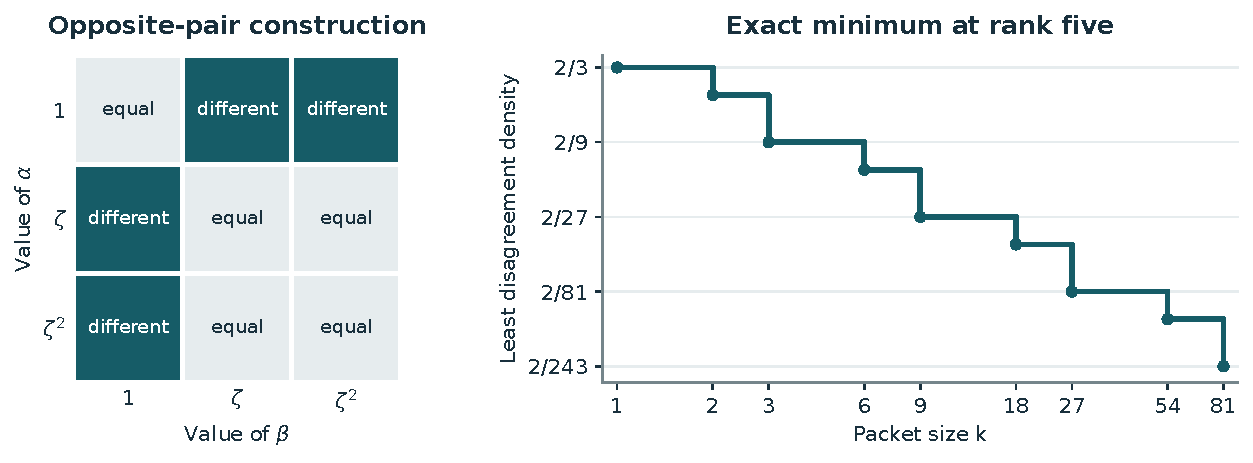
\includegraphics[width=\linewidth]{figures/cubic_staircase.pdf}
\caption{Left: the four disagreeing classes for the basic opposite-pair
construction, among nine ternary value pairs. Right: the exact minimum
disagreement as the packet size grows, at rank five; both axes are
logarithmic. The two steps per power of three reflect odd and even
Eisenstein valuations.}
\label{fig:cubic}
\end{figure}

\begin{center}
\begin{tabular}{@{}ccc@{}}
\toprule
Packet size $k$ & Least disagreement & Greatest agreement\\
\midrule
1 & $2/3$ & $1/3$\\
2 & $4/9$ & $5/9$\\
3--5 & $2/9$ & $7/9$\\
6--8 & $4/27$ & $23/27$\\
9--17 & $2/27$ & $25/27$\\
18--26 & $4/81$ & $77/81$\\
27--53 & $2/81$ & $79/81$\\
54--80 & $4/243$ & $239/243$\\
\bottomrule
\end{tabular}
\end{center}
\noindent The table holds without saturation, for example at rank $r\ge5$.
At smaller ranks, the density stops decreasing at $2/3^r$.

\section{Unequal precision in branch observations}
\label{sec:unequal-branches}

This section proves a second, unconditional extension of the source article.
Question \texttt{lub:q:adversarial} of \cite{article} asks for the branch-recovery results to be extended
to unequal truncation lengths and to coefficients modulo higher powers of a
uniformizer.  We resolve the unequal-length part over a field, including the
exact observation kernel, the complete error/erasure criterion, an exact
contact-tree algorithm, and optimal total recording budgets.  Coefficients in
$\mathcal O/\pi^r$ for $r>1$ are outside the theorem.

\subsection{The kernel and the recoverable jet}

Let $F$ be a field, put $R=F[[X]]$ and $\mathfrak m=(X,Y)$, and let
$u_b\in XR$, $b\in I$, be $N$ pairwise distinct branches.  Set
\[
 s_{bc}=\operatorname{ord}_X(u_b-u_c)\ge1\quad(b\ne c).
\]
Choose arbitrary integers $n_b\ge0$.  A branch with $n_b=0$ has an empty record.
The observations of an otherwise unrestricted $H\in F[[X,Y]]$ are
\[
 \Omega_{\boldsymbol n}(H)_b
   =H(X,u_b(X))\bmod X^{n_b}.
\]
The target is the complete total-degree jet
$J_d(H)=H\bmod\mathfrak m^d$, not merely the coefficients of a polynomial in $Y$.
It has $d(d+1)/2$ scalar coefficients.

Order the branches as follows.  Having chosen $b_0,\ldots,b_{j-1}$, choose an
unused $b_j$ maximizing
\begin{equation}
 \mu_j=n_{b_j}-\sum_{i<j}s_{b_jb_i},
 \qquad
 \Pi_j(Y)=\prod_{i<j}(Y-u_{b_i}(X)).
 \label{eq:unequal-greedy}
\end{equation}
All ties are allowed.  The scores may be negative; write
$\mu_j^+=\max(0,\mu_j)$.  Every unused score falls by at least one at the next
step, so
\begin{equation}
 \mu_{j+1}\le\mu_j-1.
 \label{eq:unequal-descent}
\end{equation}

\begin{theorem}[Exact kernel at unequal precisions]
\label{thm:unequal-kernel}
As an $R$-module, the observation kernel is
\begin{equation}
 \ker\Omega_{\boldsymbol n}
 =\Pi_N F[[X,Y]]\ \oplus\!
   \bigoplus_{j=0}^{N-1}X^{\mu_j^+}R\Pi_j.
 \label{eq:unequal-kernel}
\end{equation}
For $1\le d\le N$, the records determine $J_d(H)$ for every $H$ if and only if
\begin{equation}
 \mu_{d-1}>0.
 \label{eq:unequal-clean}
\end{equation}
The largest completely recoverable jet order is the number of positive scores.
Moreover, the dimension of the unresolved part of the target is exactly
\begin{equation}
 \dim_F\frac{\ker\Omega_{\boldsymbol n}+\mathfrak m^d}{\mathfrak m^d}
 =\sum_{j=0}^{d-1}\max\{0,d-j-\mu_j^+\}.
 \label{eq:unequal-dimension}
\end{equation}
The nonnegative exponents $\mu_j^+$ are independent of the choices at ties.
\end{theorem}

\begin{proof}
Successive division by $Y-u_{b_i}(X)$ gives a unique expansion
\[
 H=\Pi_N Q+\sum_{j<N}c_j(X)\Pi_j(Y),\qquad c_j\in R.
\]
This division is valid for formal series: $u_b\in XR$ makes substitution
well defined, and
$Y^a-u_b^a=(Y-u_b)\sum_{t=0}^{a-1}Y^{a-1-t}u_b^t$ gives the quotient term by
term in the $\mathfrak m$-adic topology.  Uniqueness of the remainder follows
by evaluating successively at $u_{b_0},u_{b_1},\ldots$; the relevant products
of distinct branch differences are nonzero in the domain $R$.

For each $j$, the function $X^{\mu_j^+}\Pi_j$ satisfies every observation
constraint.  It vanishes identically on the previously selected branches.
At any remaining branch $b$, the maximality in
\eqref{eq:unequal-greedy} gives
\[
 \mu_j^+ +\sum_{i<j}s_{bb_i}\ge n_b.
\]
Conversely suppose the remainder is in the kernel.  Evaluation at $b_0$
forces $v_X(c_0)\ge n_{b_0}=\mu_0$.  Subtract this term, which itself lies
in the kernel.  At step $j$ the previously removed terms satisfy all
constraints and the later Newton factors vanish at $b_j$, so
\[
 v_X(c_j)+\sum_{i<j}s_{b_jb_i}\ge n_{b_j}.
\]
Together with $c_j\in R$ this is $v_X(c_j)\ge\mu_j^+$.  The two implications
prove \eqref{eq:unequal-kernel}.

The Newton change of basis respects total degree.  The coefficient of $Y^i$
in $\Pi_j$, for $i<j$, belongs to $X^{j-i}R$, whereas $\Pi_j$ is monic of
$Y$-degree $j$.  Consequently
\[
 \operatorname{ord}_{\mathfrak m}\Bigl(\sum_{j<N}c_j\Pi_j\Bigr)
   =\min_{j<N}\{v_X(c_j)+j\}.
\]
For the converse inequality in this equality, among the summands of least
total order take the one with largest $Y$-degree: its leading coefficient
cannot cancel with any of the other leading forms.  Also
$\Pi_N\in\mathfrak m^N$.

If $\mu_{d-1}\ge1$, \eqref{eq:unequal-descent} gives
$\mu_j+j\ge\mu_{d-1}+d-1\ge d$ for every $j<d$; all remaining factors already
have total order at least $d$.  The kernel therefore lies in
$\mathfrak m^d$.  If $\mu_{d-1}\le0$, the kernel contains $\Pi_{d-1}$, whose
total order is exactly $d-1$, proving failure.  The classes of
$X^i\Pi_j$ with $i+j<d$ form a basis of the target jet, so counting the
kernel basis classes gives \eqref{eq:unequal-dimension}.

Finally, within the $R$-module of kernel polynomials of $Y$-degree at most
$j<N$, the possible leading coefficients form the intrinsic ideal
$X^{\mu_j^+}R$.  This ideal does not depend on the ordering and proves
tie independence of the capped scores.
\end{proof}

When all $n_b=n$, the rule is ordinary $P$-ordering, and
$\mu_j=n-\lambda_j$, where $\lambda_j$ is the greedy contact sequence of the
source article.  Thus the theorem specializes exactly to
\texttt{lub:thm:kernel}.  The weights $n_b$ cannot be replaced by their
minimum or average without losing information.

\subsection{A sparse certificate and the exact recording budget}

\begin{corollary}[Only $d$ clean branches are needed]
\label{cor:unequal-certificate}
The full observations recover $J_d$ if and only if some $d$-element subset
$S\subseteq I$ satisfies
\begin{equation}
 n_b\ge1+\sum_{c\in S\setminus\{b\}}s_{bc}\qquad(b\in S).
 \label{eq:unequal-certificate}
\end{equation}
When recovery holds, the first $d$ branches in
\eqref{eq:unequal-greedy} give such a subset.
\end{corollary}

\begin{proof}
The first $d$ choices remain a greedy order when the process is restricted
to that $d$-element set, with the same first $d$ scores.  By
Theorem~\ref{thm:unequal-kernel}, its observations recover $J_d$ whenever
those of the whole set do.

For exactly $d$ branches put
$\Delta_b=\prod_{c\ne b}(u_b-u_c)$ and $\sigma_b=v_X(\Delta_b)$.
Lagrange interpolation of the remainder of $H$ modulo
$\prod_{b\in S}(Y-u_b)$ gives
\[
 R_H(Y)=\sum_{b\in S}\frac{H(X,u_b)}{\Delta_b}
                  \prod_{c\in S\setminus\{b\}}(Y-u_c).
\]
If all records vanish and $n_b\ge\sigma_b+1$, each quotient is in $XR$;
hence every summand belongs to $\mathfrak m^d$.  If $n_b\le\sigma_b$ for
some $b$, the explicit function
\[
 \frac{X^{\sigma_b}}{\Delta_b}
       \prod_{c\in S\setminus\{b\}}(Y-u_c)
\]
is integral, has a nonzero jet of order $d$, vanishes on the other branches,
and has value $X^{\sigma_b}$ on $b$.  It is indistinguishable from zero.
This proves the necessary and sufficient componentwise criterion.
\end{proof}

One may choose the precisions before observing $H$.  The recording cost is
$\sum_b n_b$; unrecorded branches have precision zero.

\begin{theorem}[Minimum cost of clean jet recovery]
\label{thm:unequal-budget}
For fixed distinct branches and $1\le d\le N$, the least total recording
cost that recovers $J_d$ is
\begin{equation}
 B_d=d+2\min_{\substack{S\subseteq I\\|S|=d}}
                    \sum_{\{b,c\}\subseteq S}s_{bc}.
 \label{eq:unequal-budget}
\end{equation}
If $\lambda_j$ is the ordinary minimum-contact $P$-ordering sequence on all
branches, this is also
\[
 B_d=d+2\sum_{j=0}^{d-1}\lambda_j.
\]
Choose the first $d$ branches of an ordinary $P$-ordering, give each the
precision in the right side of \eqref{eq:unequal-certificate}, and give all
other branches precision zero.  This attains the minimum.
\end{theorem}

\begin{proof}
Corollary~\ref{cor:unequal-certificate} supplies a $d$-element set $S$ for
any successful profile, and summing its necessary componentwise bounds gives
$\sum_b n_b\ge d+2\sum_{\{b,c\}\subseteq S}s_{bc}$.
The same componentwise bounds show that the profile constructed from any
minimizing $S$ succeeds with exactly that cost.

For completeness, ordinary $P$-ordering attains the displayed pair-energy
minimum.  Let $a_0,a_1,\ldots$ be such an ordering, let
$P_j(Y)=\prod_{i<j}(Y-u_{a_i})$, and let $\alpha_j=P_j(u_{a_j})$, so
$v_X(\alpha_j)=\lambda_j$.  By its greedy definition every
$P_j/\alpha_j$ is integral valued on every branch.  For any $d$-element set
$S$, the evaluation matrix of $1,P_1/\alpha_1,\ldots,P_{d-1}/\alpha_{d-1}$
on $S$ has integral entries.  Its determinant is a Vandermonde determinant
divided by $\prod_{j<d}\alpha_j$, whence
\[
 \sum_{\{b,c\}\subseteq S}s_{bc}\ge\sum_{j<d}\lambda_j.
\]
For $S=\{a_0,\ldots,a_{d-1}\}$ the matrix is triangular with diagonal one,
so equality holds.
\end{proof}

\subsection{Arbitrary corrupted or erased branch records}

The block distance between distinct target jets is
\[
 \delta_d(\boldsymbol n;I)
   =\min_{H\notin\mathfrak m^d}
          \#\{b:\Omega_{\boldsymbol n}(H)_b\ne0\}.
\]
For a subset $S$, rerun \eqref{eq:unequal-greedy} with its inherited
precisions and write its scores as $\mu_j(S)$, setting
$\mu_j(S)=-\infty$ for $j\ge|S|$.  Define
\[
 C_I(j,T)=\max\{|S|:S\subseteq I,\ \mu_j(S)\le T\}.
\]
For the distance formula only $T=0$ is needed.

\begin{theorem}[Exact error and erasure threshold]
\label{thm:unequal-errors}
For $1\le d\le N$,
\begin{equation}
 \delta_d(\boldsymbol n;I)=N-C_I(d-1,0).
 \label{eq:unequal-distance}
\end{equation}
The target jet is uniquely determined for every $H$ despite at most $w$
arbitrarily corrupted blocks and at most $z$ flagged erased blocks if and
only if
\begin{equation}
 2w+z<\delta_d(\boldsymbol n;I).
 \label{eq:unequal-errors}
\end{equation}
All failures have explicit witnesses in $F[[X]][Y]$ of $Y$-degree at most
$d-1$ and total order at most $d-1$.  Finite polynomial witnesses result
by truncating their $X$-coefficients sufficiently far.
\end{theorem}

\begin{proof}
If $|S|\ge d$, Theorem~\ref{thm:unequal-kernel} gives a nonzero target jet
whose observations vanish on $S$ exactly when $\mu_{d-1}(S)\le0$.
In this case $\Pi_{d-1}$ for the greedy order on $S$ is a witness.
For $|S|<d$, the product $\prod_{b\in S}(Y-u_b)$ is a witness at every
precision.  Thus $C_I(d-1,0)$ is exactly the largest possible zero set of
an observation word with nonzero target, proving
\eqref{eq:unequal-distance}.

Two explanations of the same received records differ on at most the
union of their error locations and the erased locations, namely $2w+z$
blocks.  If this is smaller than the target distance, their target jets
coincide.  Conversely choose a minimum-distance word with nonzero target
and compare it with zero.  If $\delta_d\le2w+z$, erase up to $z$ of its
nonzero blocks and partition the remaining at most $2w$ blocks into two
sets of size at most $w$.  On one set let the received word agree with
zero, and on the other let it agree with the chosen word.  Both target
jets then explain the data.  When $\delta_d=0$, the ambiguity exists even
without errors.  To obtain a finite polynomial witness, truncate each
$X$-coefficient at $M=\max\{d,n_{\max}\}$, where
$n_{\max}=\max_b n_b$.  The discarded terms belong to $X^MF[[X,Y]]$;
they affect neither the target jet nor any record.
\end{proof}

This is a target-jet distance: words caused solely by terms of total degree
at least $d$ need not have positive distance.  It is therefore not legitimate
to replace it by the minimum distance of the entire observation code.

\begin{corollary}[Exact componentwise saturation and its cost]
\label{cor:unequal-saturation}
Always $\delta_d\le N-d+1$.  Equality holds if and only if, for each $b$,
\begin{equation}
 n_b\ge 1+
     \text{the sum of the $d-1$ largest numbers $s_{bc}$, $c\ne b$}.
 \label{eq:unequal-saturation}
\end{equation}
The least total recording cost attaining distance $N-d+1$ is the sum of
these $N$ componentwise lower bounds.  In particular, if
$N=d+2w+z$, this is exactly the minimum cost of correcting $w$ corrupted
blocks and $z$ erased blocks.
\end{corollary}

\begin{proof}
A product of $d-1$ branch equations has a nonzero target and vanishes on
those branches, proving the upper bound.  Equality is equivalent to
clean recovery from every $d$-element subset.  Apply
\eqref{eq:unequal-certificate} to each such subset and maximize the sum
of contacts at each fixed $b$.  The resulting inequalities are independent
componentwise lower bounds and attain equality simultaneously.  When
$N=d+2w+z$, condition \eqref{eq:unequal-errors} requires the maximum
possible distance $N-d+1$.
\end{proof}

\subsection{The exact contact-tree algorithm}

The contact numbers satisfy
$s_{bc}\ge\min\{s_{ba},s_{ac}\}$.  Represent them by a rooted tree whose
leaves are the branches: the common path length of two distinct leaves is
their contact.  The root has a stem of length $\min s_{bc}$; a nonleaf
cluster splits according to strict increase of contact.  Let $\ell_v$ be
the incoming length of a node, let $I_v$ be its leaves, and use the residual
contact lengths below its parent.  At a leaf put $\mu_0^v=n_b$ and
$\mu_j^v=-\infty$ for $j\ge1$.

\begin{lemma}[Weighted merge]
\label{lem:unequal-merge}
Let $z_0\ge z_1\ge\cdots$ be the decreasing rearrangement of the union of
the finite score lists of the children of $v$.  Then
\[
 \mu_j^v=z_j-j\ell_v\qquad(0\le j<|I_v|).
\]
In particular the full score list, including its negative entries, depends
only on the contact tree and the precision labels, and not on tie choices.
\end{lemma}

\begin{proof}
After $j$ choices every remaining candidate pays the same $j\ell_v$
for the common stem.  Its remaining penalty involves only choices in its
own child.  Each child offers a nonincreasing stream of scores, by
induction from the leaves.  The maximum rule therefore merges those
streams in decreasing order and subtracts $j\ell_v$ at step $j$.
\end{proof}

Define
\[
 C_v(j,T)=\max\{|S|:S\subseteq I_v,\ \mu_j^v(S)\le T\},
\]
again using $-\infty$ beyond the finite score list.

\begin{theorem}[Pruning recursion]
\label{thm:unequal-tree}
If $j\ge|I_v|$ or $T\ge\max_{b\in I_v}n_b$, then $C_v(j,T)=|I_v|$.
For a leaf $b$,
\[
 C_b(0,T)=\begin{cases}1,&n_b\le T,\\0,&n_b>T,\end{cases}
 \qquad C_b(j,T)=1\quad(j\ge1).
\]
At an internal node,
\begin{equation}
 C_v(j,T)=
 \max_{\substack{j_c\ge0\\\sum_c j_c\le j}}
       \sum_c C_c(j_c,T+j\ell_v).
 \label{eq:unequal-pruning}
\end{equation}
Backtracking maximizing allocations gives a maximal zero set and therefore
a sharp ambiguity witness in Theorem~\ref{thm:unequal-errors}.
For scores up to $d-1$, a direct integer-threshold implementation uses
$O(Nd^2(n_{\max}+1))$ elementary arithmetic operations, where
$n_{\max}=\max_b n_b$; all larger thresholds can be capped.
\end{theorem}

\begin{proof}
By Lemma~\ref{lem:unequal-merge}, including the $-\infty$ tail,
$\mu_j^v(S)\le T$ is equivalent to the $j$th entry of the merged child
streams being at most $T+j\ell_v$.  This says that at most $j$ entries
of those streams are strictly greater than that threshold.  If child
$c$ contributes $h_c$ such entries, then $\sum_c h_c\le j$, and
$h_c\le j_c$ is exactly the condition
$\mu_{j_c}^c(S\cap I_c)\le T+j\ell_v$.  This gives both directions of
\eqref{eq:unequal-pruning} by taking maximizing sets in the children.
The base cases are immediate.  Starting at $T=0$, thresholds never
become negative; a threshold at least $n_{\max}$ imposes no restriction.
There are $O(N)$ nodes in the compact contact tree, $d$ ranks and at
most $n_{\max}+1$ relevant integer thresholds.  For each child threshold $U$, combine the child tables for all rank
budgets simultaneously by max-convolution, at cost $O(d^2)$ per child.
The table entry $(j,T)$ at the parent then reads the resulting rank-$j$
entry at $U=\min\{n_{\max},T+j\ell_v\}$.  This proves the operation bound.
\end{proof}

The algorithm computes the exact distance and a worst surviving
configuration.  It is not a polynomial-time decoder for corrupted records:
one may still decode by enumerating candidate error sets and solving finite
linear systems, and the faster error-location part of the source question
remains open here.

\subsection{Two exact examples and verification}

Over $F=\mathbb F_2$, take $u_b=(1+X)^b-1$ for $0\le b\le7$ and precisions
\[
 (n_0,\ldots,n_7)=(6,4,9,5,8,3,7,4).
\]
The contacts are $s_{bc}=2^{v_2(b-c)}$.  Breaking ties by the smallest
index, the greedy order and scores are
\[
 (2,4,3,1,6,0,7,5),\qquad(9,6,3,0,-1,-4,-6,-9).
\]
Thus the $46$ recorded coefficients recover the complete order-three jet,
consisting of the six coefficients of $1,X,Y,X^2,XY,Y^2$, but do not
recover the order-four jet.  The exact order-three distance is $4$, so
one arbitrary corrupt record together with one flagged erased record
is correctable.  Two arbitrary corruptions cannot always be corrected.
A sharp nonzero difference is
\[
 H(X,Y)=Y(Y+X+X^2+X^3).
\]
Its records vanish on branches $0,3,5,7$ and are nonzero precisely on
$1,2,4,6$.

For an exact allocation example, work over $\mathbb F_5$ with branches
\[
 0,\quad X^5,\quad X,\quad2X,\quad3X.
\]
The first two have contact $5$; every other pair has contact $1$.
For the order-three jet, the least componentwise profile giving maximal
distance $3$ is
\[
 (7,7,3,3,3).
\]
Its total cost is $23$, and it corrects one arbitrary corrupted branch.
Every successful profile for this five-branch, one-corruption problem has
cost at least $23$.  A common precision needs $7$ coefficients at every
branch, costing $35$.

The accompanying script \texttt{verify\_unequal\_branches.py} verifies the
claims using exact finite-field arithmetic.  It exhausts all $5^4=625$
precision profiles with values $0,\ldots,4$ on four binary multiplicative
branches; adds $120$ deterministic random configurations over
$\mathbb F_2,\mathbb F_3,\mathbb F_5$; and checks the two displayed examples.
Across these $747$ profiles it performs $2{,}996$ comparisons of the
unresolved-jet formula against direct expansion and matrix rank,
$2{,}996$ comparisons of the tree recursion against exhaustive branch
subsets, and $2{,}996$ checks of the componentwise saturation criterion.
These finite checks corroborate the proof; they are not substitutes for it.

\subsection{Attribution and scope of novelty}

The use of Newton polynomials and $P$-orderings is classical
\cite{bhargava}.  Weighted greedy selection on an ultrametric is likewise
established: Grinberg and Petrov \cite{grinbergpetrov} treat element weights
and ultrametric pair contributions.  The rule here is their greedy
perimeter rule with weight $n_b$ and pair distance $-s_{bc}$.
Amini \cite{amini} supplies the related unweighted tree-factorial framework.

The contribution claimed here is the exact unequal-truncation observation
kernel for unrestricted bivariate formal series, its total-degree target
interpretation, and the resulting sharp deletion/error and recording-budget
formulas.  These resolve the specified unequal-length question in the
supplied article.  A targeted literature search found no prior statement of
this combined recovery result, but that is not a proof of worldwide priority.
The seven ZIP reports in the repository's incoming directory at the pinned
commit were also checked; none states this extension.  No assertion is made
that $P$-orderings, weighted greedy optimality, Lagrange interpolation, or the
standard distance inequality $2w+z<\delta$ are new.

\section{Verification, reproducibility, and remaining scope}
\label{sec:verification}

\subsection{What was checked exactly}

The general assertions are proved in the preceding sections. The finite
checks test independent formulations and boundary cases; they do not
establish the theorems by extrapolation. All arithmetic in the substantive
verification scripts is exact.

\begin{center}
\small
\begin{tabularx}{\linewidth}{@{}L{0.34\linewidth}YL{0.18\linewidth}@{}}
\toprule
Check & Scope & Outcome\\
\midrule
Exhaustive cubic packet comparison &
$r=1$, $k=1,\ldots,8$; $r=2$, $k=1,\ldots,6$;
$r=3$, $k=1,2,3$; $r=4$, $k=1,2$ &
17\,735\,976 pairs; all agree\\[3pt]
Extremizer structure & Translation periods and quotient forms, including
repeated saturated entries & 5285 extremizers checked\\[3pt]
Eisenstein local cost & Nonzero zero-sum triples of positive mass at most
300 & 270\,900 triples checked\\[3pt]
Sharp constructions and Fourier norms & Two- and four-coset constructions
through rank six & 36 constructions checked\\[3pt]
Independent cubic implementation & Separate local multiplicity enumeration
in 13 small parameter cases & 1\,036\,722 pairs; all agree\\[3pt]
Unequal branch recovery & 625 exhaustive profiles, 120 seeded finite-field
examples, two displayed examples & 747 profiles checked\\[3pt]
Direct branch matrix ranks & Compare unresolved-jet dimensions using exact
finite-field elimination & 2996 comparisons pass\\[3pt]
Pruning and saturation & Compare tree recursion with all branch subsets;
check the componentwise distance criterion & 2996 checks each pass\\
\bottomrule
\end{tabularx}
\end{center}

The independent cubic implementation does not use Eisenstein valuations
or Reed--Muller weights. It compares the three local-root multiplicities
directly, so its agreement with the density theorem tests a different
description. The principal implementation also checks the proposed
extremizer families using their translation stabilizers. Structural checks
were capped at 500 extremal pairs per parameter case; the minimum-density
comparison itself includes every pair in the displayed ranges.

For branches, direct expansion and row reduction determine the ambiguity
of the target jet after allowing unrestricted higher terms up to the
finite observation cutoff. A separate contact-tree computation is checked
against enumeration of all retained subsets. The finite-field runs also
check 1423 successful sparse recovery certificates. They use fixed seed
\code{20261127}; no random floating-point linear algebra is involved.

An independent agent reviewed both mathematical arguments adversarially.
The reviews are included in the archive. One wording error was corrected:
branch ambiguity witnesses have small $Y$-degree and small total
\emph{order}; their total degree need not be small. This matters when a
branch contains high powers of $X$. The final manuscript states the
correct property and explains finite polynomial truncation.

\begin{figure}[htbp]
\centering
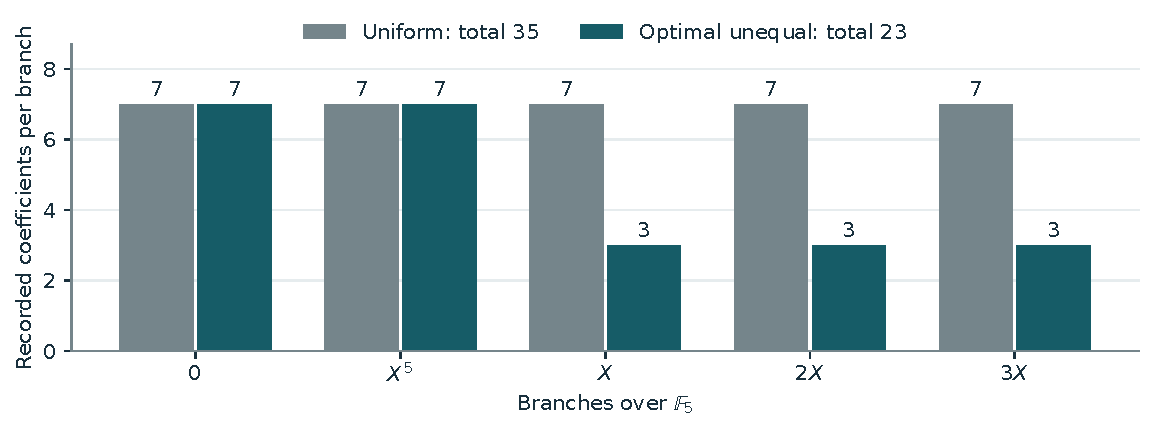
\includegraphics[width=0.92\linewidth]{figures/precision_budget.pdf}
\caption{The sharp five-branch allocation example over $\F_5$.
Both allocations recover the order-three jet despite one arbitrary
corrupted record. The unequal profile uses 23 coefficients; every uniform
profile with the same guarantee uses at least 35.}
\end{figure}

\subsection{Rebuilding and interpreting the artifacts}

The archive contains the main \code{report.tex}, its chapter sources,
compiled \code{report.pdf}, bibliography, verification code, JSON outputs,
figure sources and outputs, provenance, and proof-review notes.
The \code{Makefile} provides the following targets:
\begin{itemize}
\item \code{make pdf}: compile the manuscript with \code{latexmk};
\item \code{make verify}: rerun the exact mathematical checks;
\item \code{make figures}: regenerate publication figures from the stated
formulas and recorded exact examples;
\item \code{make source-audit SOURCE=/path/to/ProveIt}: rerun the local
source scan against a separately obtained checkout.
\end{itemize}
Both cubic verifiers use NumPy; the branch verifier uses only the Python
standard library. The delivered results record the
actual test environment. A full upstream source checkout and third-party
papers are not copied into the archive. Pinned links and a file manifest
identify what was read. Rebuilding the new manuscript or rerunning its
finite checks does not build the upstream Lean project.

\subsection{Novelty assessment and boundaries}

The exact cubic extremal function and its complete equality classification
were not found in the supplied article, its relevant recent reports, or
the seven incoming ZIP reports at the pinned revision. The proof directly
extends the article's quadratic Fourier/valuation approach. The new
features are the two Eisenstein valuation costs, the parity obstruction to
an even minimum support, and the resulting sharp packet classifications.
Known coding theorems are explicitly cited, and the generic
$k^2\log^2 Q$ detection scale is not claimed as new.

Targeted primary-literature searches covered cubic-character matching,
integral ternary Fourier uncertainty, and finite-group character matching.
Walji's matching-density work and Martin--Walji's character comparison
results address adjacent representation-theoretic questions
\cite{walji2016,martinwalji2017}; they do not state the reducible cubic
packet classification proved here. The second extension explicitly
credits weighted greedy selection to established work
\cite{grinbergpetrov}. A search that does not find an exact predecessor
does not establish worldwide priority. These results should be treated
as proved research contributions relative to the supplied collection,
with priority subject to further expert literature review.

The following tasks are not settled here: the full cubic nonextremal
density spectrum, the matching problem for every odd prime exponent,
mixed coefficient rings $\mathcal O/\pi^r$ with $r>1$, and a fast
error-location decoder. The dynamic program computes the exact
branch distance and extremal deletion set; it does not by itself locate
corrupted records from arbitrary received values.

Finally, none of the new theorems is a Lean-certified extension of the
vendor package. The document gives mathematical proofs and reproducible
exact checks. The appendix describes how a future formalization can be
separated into finite algebraic work and the single analytic interface.

\appendix
\section{Formalization plan and dependency separation}
\label{sec:formalization}

This appendix is a plan, not a collection of machine-checked declarations.
No uncompiled Lean file with placeholder proof terms is presented as a
proof artifact.

\subsection{Finite cubic theorem}

The main algebraic theorem can be formalized independently of analytic
$L$-functions. Start with the finite type $X=\F_3^r$, its dual $V$, and
a nonzero coefficient function $c:X\to\Z$ with zero sum. Define its
positive mass and the transform in the Eisenstein integers. A natural
dependency order is:
\begin{enumerate}
\item Finite Fourier orthogonality and inversion; support symmetry and
the zero value at the identity.
\item The zero-sum triple lemma, including the exact odd/even
$1-\zeta_3$ valuations and their mass bounds.
\item Coordinate interpolation on $\{0,1,2\}$ over the Eisenstein ring
with 2 inverted; coefficient divisibility and reduction to a low-degree
ternary polynomial.
\item The needed minimum and second-weight Reed--Muller theorems,
including the affine support-containment statements. Their mathematical
citations are explicit, but availability as matching Lean declarations
has not been established in this session.
\item The piecewise lower bound, exact coset constructions, and all
equality cases via Fourier inversion.
\end{enumerate}
Steps 1--5 yield a purely finite theorem. Its Dirichlet interpretation
then needs surjectivity of the residue-class evaluation map and the prime
number theorem in arithmetic progressions. The finite-prime statements
separately need the smoothed explicit-formula interface and the exported
Dirichlet GRH. The imported GRH does not automatically formalize those
intermediate estimates.

\subsection{Branch recovery}

The second development can also be kept independent of GRH. Its core is
formal substitution and division in $F[[X,Y]]$, the discrete valuation on
$F[[X]]$, a finite weighted greedy ordering, and an exact Newton basis.
After the kernel identity, filtered linear algebra gives the target-jet
dimension and recovery criterion. Lagrange interpolation supplies the
$d$-branch certificate and sharp recording budgets.

The error/erasure theorem should be formalized for the quotient target
explicitly. Two different source series may have the same target jet,
so ordinary injectivity of the whole observation map is the wrong
specification. One can define target distance as the smallest support of
an observation word arising from a series outside $(X,Y)^d$, then prove
the distance criterion and the tree recursion.

\subsection{What the supplied Lean theorem does and does not discharge}

After the finite and analytic interfaces above have been formalized,
the supplied declaration
\begin{center}
\code{LFunction\_ne\_zero\_of\_half\_lt\_re}
\end{center}
or the critical-strip theorem can discharge the Dirichlet-GRH hypothesis of
the counting results. It is unnecessary for the exact extremal density
or branch-kernel theorems. Neither the absence of forbidden tokens in
the vendor source nor the success of the finite Python checks should be
used as a substitute for this future formal proof.

\clearpage
\bibliographystyle{plain}
\bibliography{references}
\end{document}
